% IV-2-2 · БД1 тайлан. Хөрвүүлэх:  cd report && xelatex IV-2-2_BD1_Report.tex (2 удаа — агуулга)
% Шаардлага: texlive-xetex, fonts-dejavu (Ubuntu: sudo apt install texlive-xetex texlive-lang-cyrillic fonts-dejavu)
\documentclass[11pt,a4paper]{article}
\usepackage{fontspec}
\setmainfont{DejaVu Serif}
\setsansfont{DejaVu Sans}
\setmonofont{DejaVu Sans Mono}[Scale=0.82]
\usepackage[margin=2.1cm]{geometry}
\usepackage{graphicx}
\usepackage{xcolor}
\usepackage{enumitem}
\usepackage{booktabs}
\usepackage{longtable}
\usepackage{array}
\usepackage{listings}
\usepackage{tikz}
\usetikzlibrary{arrows.meta,positioning,fit,backgrounds}
\usepackage{hyperref}
\usepackage{titlesec}
\usepackage{caption}
\usepackage{placeins}

\titleformat{\section}{\Large\bfseries}{\thesection.}{0.5em}{}
\titleformat{\subsection}{\large\bfseries}{\thesubsection}{0.5em}{}
\setlength{\parskip}{0.45em}
\setlength{\parindent}{0pt}
\sloppy
\setlength{\emergencystretch}{3em}
\hypersetup{colorlinks, linkcolor=blue!50!black, urlcolor=blue!50!black,
  pdftitle={IV-2-2 BD1 Report: Linux Kernel Module for Task Information}}
\captionsetup{font=small, labelfont=bf}
\graphicspath{{../docs/images/}{../src/ui/screenshots/}}

\lstset{
  basicstyle=\ttfamily\small, keywordstyle=\color{blue!70!black}\bfseries,
  commentstyle=\color{green!45!black}, stringstyle=\color{red!60!black},
  frame=single, framerule=0.3pt, rulecolor=\color{gray!60}, backgroundcolor=\color{gray!6},
  columns=fullflexible, keepspaces=true, language=C, showstringspaces=false,
  xleftmargin=0.5em, xrightmargin=0.5em, breaklines=true
}
\lstdefinestyle{out}{language={}, backgroundcolor=\color{black!3}}
\newfontfamily\symfont{DejaVu Sans}
\newcommand{\ok}{{\symfont\textcolor{green!50!black}{✔}}}
\newcommand{\warn}{{\symfont\textcolor{orange!80!black}{⚠}}}
\newcommand{\no}{{\symfont\textcolor{red!70!black}{✖}}}
\renewcommand{\contentsname}{Агуулга}
\renewcommand{\figurename}{Зураг}
\renewcommand{\tablename}{Хүснэгт}
\newcommand{\pass}{\textcolor{green!50!black}{\textbf{PASS}}}
\DeclareRobustCommand{\code}[1]{\texttt{\detokenize{#1}}}

\begin{document}

%================================================================ Нүүр
\begin{titlepage}
\centering
\vspace*{1.2cm}
{\large ШИНЖЛЭХ УХААН ТЕХНОЛОГИЙН ИХ СУРГУУЛЬ\\ Мэдээлэл, Холбооны Технологийн Сургууль\par}
\vspace{2cm}
{\large F.CSM302 Үйлдлийн систем — Бие даалт 1\par}
\vspace{0.8cm}
{\Huge\bfseries Linux Kernel Module for Task Information\par}
\vspace{0.4cm}
{\Large \code{/proc/pid} ба Task hierarchy дүрслэл\par}
\vspace{1cm}
{\large Судалгаа, хэрэгжилт, туршилтын тайлан\par}
\vspace{1.6cm}
\begin{tabular}{r p{10cm}}
\textbf{Хуваарилалтын код:} & IV-2-2\\
\textbf{Сурах бичиг:} & Silberschatz, Galvin, Gagne — OSC (2018), 3-р бүлэг, Programming Project 2\\
\textbf{UI дүрслэл:} & Task hierarchy (parent – task – children мод)\\
\textbf{Repository:} & \url{https://github.com/Tugu8/os-bd1-IV-2-2-}\\
\textbf{Багш:} & Доктор (Ph.D) Г. Ганбат\\
\end{tabular}
\vspace{1.2cm}

\begin{tabular}{l p{12cm}}
\toprule
\textbf{Гишүүн} & \textbf{Хариуцсан хэсэг}\\
\midrule
B242270047 & Kernel module (\code{src/kmod/})\\
B190910014 & Interactive UI (\code{src/ui/})\\
B210930842 & Бэлтгэл module, build орчин, Operational manual (\code{src/prereq/})\\
B231910003 & Туршилт (\code{tests/})\\
B232270108 & Үндсэн тайлан (\code{report/})\\
B241940099 & Хэрэглэгчийн manual, README Quick Start, БД1 пост, шүүмж (\code{review/})\\
\bottomrule
\end{tabular}

\smallskip
{\small Тайланг бэлтгэсэн: B190910014 · хянаж баталгаажуулах: B232270108}
\vfill
{\large 2026 оны 10-р сар\par}
\end{titlepage}

%================================================================ Хураангуй
\section*{Хураангуй}
\addcontentsline{toc}{section}{Хураангуй}

\textbf{Асуудал.} Хэрэглэгчийн орон зайн программ процессын мэдээллийг (PCB буюу \code{struct task_struct}) шууд уншиж чадахгүй. Сурах бичгийн 3-р бүлгийн Programming Project 2 нь \code{/proc/pid} виртуал файлаар PID хүлээн авч, тухайн task-ийн нэр, PID, төлөвийг буцаадаг kernel module бичихийг шаарддаг. Багшийн оноосон дүрслэл нь сонгосон процессын эцэг, хүүхдүүдийг шатлалтай мод хэлбэрээр харуулах \emph{task hierarchy} юм.

\textbf{Шийдэл.} \code{pid.ko} module нь \code{/proc/pid}-д бичсэн PID-ийг \code{kstrtol}-оор шалгаж хадгална. Уншихад \code{seq_file}-ээр номын яг форматтай мөр (\code{command = [..] pid = [..] state = [..]}), дараа нь \code{parent} ба \code{child} мөрүүдийг хэвлэнэ. Python стандарт сан дээрх вэб сервер module-тэй \code{/proc/pid}-ээр харилцаж, SVG мод, төлөвийн өнгө, өөрчлөлтийн тодруулга, туршилтын процессын модыг харуулна.

\textbf{Туршилт.} Номын жишээ (bash, PID 1), байхгүй PID, 7 төрлийн буруу оролт, kernel thread, хүү процесс үүсгэх тестүүдийг bare-metal Ubuntu 24.04 (kernel 7.0.0) болон хөгжүүлэлтийн WSL2 (kernel 6.6.87.2) дээр ажиллуулсан.

\textbf{Гол үр дүн.} Bash скриптийн 11 тест, 2-р бүлгийн бэлтгэл module-ийн 9 шалгалт, UI-ийн 24 API ба 12 байрлалын тест бүгд давсан; module ↔ UI интерфейсийн шалгагч 17 \ok, 0 \no{}. Туршилтаар PID namespace-ийн алдаа (\code{task->pid} → \code{task_pid_vnr}) илэрч засагдсан.

\tableofcontents
\newpage

%================================================================ 1
\section{Удиртгал}

\textbf{Зорилго.} Linux kernel-ийн доторх процессын өгөгдлийн бүтцийг (\code{task_struct}, процессын мод) \code{/proc} файлын системээр дамжуулан хэрэглэгчид гаргаж, түүнийг интерактив мод хэлбэрээр дүрслэх.

\textbf{Ач холбогдол.} Энэ төсөл нь онолын хэд хэдэн ойлголтыг бодитоор холбоно: процесс ба PCB (OSC §3.1), процесс үүсгэх ба процессын мод (§3.3, \code{fork}, \code{wait}, zombie), kernel ба user space-ийн хил (\code{copy_from_user}), kernel module (2-р бүлэг), зэрэгцээ хандалт ба синхрончлол (RCU, мутекс — 6-р бүлэг).

\textbf{Хамрах хүрээ.}
\begin{itemize}[nosep]
  \item \code{src/prereq/} — 2-р бүлгийн бэлтгэл module-ууд: \code{simple}, \code{/proc/hello}, \code{/proc/jiffies}, \code{/proc/seconds}.
  \item \code{src/kmod/pid.c} — үндсэн module: \code{/proc/pid} write ба read, parent/children өргөтгөл.
  \item \code{src/ui/} — task hierarchy вэб UI, туршилтын процессын мод, module ↔ UI интерфейсийн шалгагч.
  \item \code{tests/} — үндсэн ба захын тест; \code{docs/Manual.md} — хэрэглэгчийн ба operational заавар.
\end{itemize}
Хамрахгүй: kernel-ээс процессын үүсэл/дуусгаврыг эвентээр мэдээлэх (UI тогтмол хугацаанд асуудаг), \code{/proc/pid}-ийг олон хэрэглэгч зэрэг ашиглах.

%================================================================ 2
\section{Сурах бичгийн шаардлага}

OSC (2018), 3-р бүлэг, Programming Project 2 ``Linux Kernel Module for Task Information'' (P-15–P-17):
\begin{enumerate}[nosep]
  \item \code{/proc/pid} файл үүсгэх module бичих.
  \item Хэрэглэгч \code{echo "1395" > /proc/pid} гэж PID бичнэ. Module оролтыг \code{kmalloc} + \code{copy_from_user}-ээр kernel санах ой руу хуулж, \code{kstrtol}-оор тоо болгон хадгална.
  \item \code{cat /proc/pid} хийхэд тухайн task-ийн \code{command}, \code{pid}, \code{state}-ийг хэвлэнэ. Task-ийг \code{pid_task(find_vpid(pid), PIDTYPE_PID)}-ээр олно.
  \item Хүчингүй PID бол \code{find_vpid} \code{NULL} буцаах тул юу ч хэвлэхгүй (read 0 байт).
\end{enumerate}

\begin{lstlisting}[style=out]
$ echo "1395" > /proc/pid
$ cat /proc/pid
command = [bash] pid = [1395] state = [1]
\end{lstlisting}

\textbf{Нэмэлт шаардлага (BD1 заавар).} Номын үндсэн функцийг бүрэн хэрэгжүүлэх; оролтыг өөрчилж дахин турших; буруу, захын оролтыг шалгах; оноосон дүрслэл бүхий UI-ийг бодит ажиллагаатай холбох; Manual-ийн дагуу өөр компьютерт дахин ажиллуулах боломж бүрдүүлэх.

%================================================================ 3
\section{Онолын үндэс}

\subsection{PCB ба \code{task_struct}}
Kernel процесс бүрийг \emph{process control block} буюу Linux-д \code{struct task_struct}-ээр (\code{<linux/sched.h>}) төлөөлнө. Энэ төсөлд ашигласан талбарууд:

\begin{center}
\begin{tabular}{>{\ttfamily}l p{11.5cm}}
\toprule
\textrm{\textbf{Талбар}} & \textbf{Утга}\\
\midrule
comm & Гүйцэтгэх файлын нэр (16 байт хүртэл)\\
\_\_state & Төлөвийн битийн маск: 0 — running, 1 — \code{TASK_INTERRUPTIBLE}, 2 — \code{TASK_UNINTERRUPTIBLE}, 4 — \code{__TASK_STOPPED}; kernel 5.14-өөс \code{state}-ийн оронд\\
real\_parent & Процессыг \code{fork} хийсэн эцэг (эцэг нь дуусвал init/subreaper руу шилжинэ)\\
children, sibling & Хүүхдүүдийн давхар холбоост жагсаалт: эцгийн \code{children} толгой, хүүхэд бүрийн \code{sibling} зангилаа\\
pid, tgid & Урсгалын ба процессын (thread group) дугаар — \emph{global} namespace-д\\
\bottomrule
\end{tabular}
\end{center}

\subsection{Процессын мод ба төлөв}
Linux-д процесс бүр (PID 0-ээс бусад) нэг эцэгтэй тул бүх процесс нэг мод үүсгэнэ: үндэс нь \code{systemd}/\code{init} (PID 1). Хүүхэд дуусахад эцэг нь \code{wait()} хийх хүртэл \emph{zombie} (\code{Z}) төлөвт үлдэнэ; эцэг нь эхэлж дуусвал хүүхэд \emph{өнчин} болж init руу шилжинэ (OSC §3.3.2). \code{ps}-ийн үсгэн төлөв (\code{R S D T Z I}) нь \code{__state} ба \code{exit_state}-ээс \code{task_state_to_char()}-аар гарна.

\subsection{\code{/proc} файлын систем}
\code{/proc} нь дискэн дээр байхгүй, санах ойд л байдаг виртуал файлын систем. \code{proc_create(name, mode, parent, &proc_ops)} нь файл үүсгэж, унших/бичих бүрт module-ийн функцийг дуудна. Kernel 5.6-аас \code{struct file_operations}-ийн оронд \code{struct proc_ops} ашиглана. Урт гаралтыг \code{seq_file} (\code{single_open}, \code{seq_printf}, \code{seq_read}) буферлэж, offset ба дахин уншилтыг зөв зохицуулна.

\subsection{Kernel ба user space-ийн хил}
User space-ийн заагч kernel-д хүчингүй эсвэл хортой байж болох тул шууд хандахгүй: \code{copy_from_user()} хаягийг шалгаж хуулна. Kernel санах ойг \code{kmalloc(…, GFP_KERNEL)}-ээр авч, бүх замд \code{kfree()} хийнэ.

\subsection{Зэрэгцээ хандалт: RCU ба мутекс}
Процессын жагсаалт байнга өөрчлөгддөг. \code{find_vpid}, \code{pid_task}, \code{real_parent}, \code{children}-ийг \code{rcu_read_lock()} дор уншиж, уншиж байх хооронд task чөлөөлөгдөхөөс сэргийлнэ (read-copy-update, OSC §6.7-ийн уншигч/бичигчийн хувилбар). Module сүүлд бичсэн PID-ийг нэг глобал \code{l_pid}-д хадгалдаг тул ``бичих → унших'' нь хоёр тусдаа систем дуудалт; хоёр процесс зэрэг ажиллавал \emph{уралдааны нөхцөл} үүснэ. UI сервер үүнийг эгзэгтэй муж болгон мутексээр хамгаална (§5.3).

\subsection{PID namespace}
Контейнер, WSL2-д процесс өөрийн PID namespace-тэй байж, нэг task өөр namespace-д өөр дугаартай байна. \code{find_vpid(n)} нь \emph{дуудагчийн} namespace-д хайдаг тул хэвлэх PID-ийг мөн дуудагчийн namespace-ээр (\code{task_pid_vnr}) гаргах хэрэгтэй.

%================================================================ 4
\section{Системийн зохиомж}

\begin{figure}[h]
\centering
\resizebox{\linewidth}{!}{%
\begin{tikzpicture}[
  box/.style={draw, rounded corners=3pt, align=center, minimum height=1cm, font=\small, fill=#1},
  box/.default=white, arr/.style={-{Stealth[length=2.2mm]}, thick}, lbl/.style={font=\scriptsize, align=center}]
  \node[box=blue!6]   (br)  {Браузер\\\scriptsize index.html, app.js, tree.js};
  \node[box=green!7, right=1.6cm of br] (srv) {\code{server.py}\\\scriptsize ThreadingHTTPServer, мутекс};
  \node[box=orange!10, right=1.6cm of srv] (proc) {\code{/proc/pid}\\\scriptsize виртуал файл};
  \node[box=red!8, below=1.8cm of proc] (mod) {\code{pid.ko}\\\scriptsize proc\_write, pid\_show};
  \node[box=gray!12, below=1.8cm of srv, xshift=-1.3cm] (ts) {\code{task_struct}\\\scriptsize comm, \_\_state, real\_parent, children};
  \node[box=gray!6, below=1.8cm of br] (pf) {\code{/proc/<pid>/stat}\\\scriptsize uid, урсгал, өвөг эцэг};
  \draw[arr] (br) -- node[lbl, above]{GET /api/task\\?pid=N} (srv);
  \draw[arr] (srv) -- node[lbl, above]{write(N)\\read()} (proc);
  \draw[arr] (proc) -- node[lbl, right]{kernel\\дуудалт} (mod);
  \draw[arr] (mod) -- node[lbl, below=2pt]{rcu\_read\_lock\\find\_vpid → pid\_task} (ts);
  \draw[arr, dashed] (srv.south west) -- node[lbl, left, pos=0.4]{uid, урсгал} (pf.north east);
  \begin{scope}[on background layer]
    \node[draw, dashed, gray, fit=(mod)(ts), inner sep=8pt, label={[font=\scriptsize, gray]below:kernel space}] {};
  \end{scope}
\end{tikzpicture}}
\caption{Компонент ба өгөгдлийн урсгал. Тасархай — procfs-оос нэмэлт мэдээлэл.}
\end{figure}

\begin{center}
\begin{tabular}{l p{11.2cm}}
\toprule
\textbf{Компонент} & \textbf{Үүрэг}\\
\midrule
\code{pid.ko} & \code{/proc/pid} үүсгэнэ; write — PID шалгаж хадгална; read — task, эцэг, хүүхдүүдийг хэвлэнэ\\
\code{server.py} & HTTP + JSON API; оролт шалгах (зөвхөн цифр, 0–4194304); write+read-ийг мутекс дотор; хүүхэд бүрийг дахин асууж \code{depth} түвшний мод үүсгэнэ (≤ 400 зангилаа)\\
Backend горим & \code{module} (\code{/proc/pid_tree}-тэй), \code{book} (зөвхөн \code{/proc/pid} — манай module), \code{fallback} (module-гүй, тодорхой тэмдэглэнэ)\\
\code{app.js}, \code{tree.js} & SVG мод (tidy tree, олон навчийг сүлжээ), өөрчлөлт харьцуулах, түүх, туршилт удирдах, экспорт\\
\code{demo_tree.py} & Мэдэгдэж буй бүтэцтэй туршилтын процессын мод (S, R, T, Z, 5 урсгалтай); signal-ийг зөвхөн энэ бүлэгт\\
\code{contract_check.py} & Module-ийн гаралтыг UI-ийн задлагчтай тулгах 18 шалгалт\\
\bottomrule
\end{tabular}
\end{center}

\textbf{Гаралтын формат (module ↔ UI гэрээ).} Эхний мөр нь номын яг формат; дараагийн мөрүүд нь hierarchy-ийн өргөтгөл. Байхгүй PID бол 0 байт.
\begin{lstlisting}[style=out]
command = [bash] pid = [5090] state = [1]
parent = [bash] ppid = [5084]
child = [sleep] pid = [5106] state = [8193]
child = [cat] pid = [5108] state = [0]
\end{lstlisting}

%================================================================ 5
\section{Хэрэгжилт}

Хэл ба сан: kernel module — C (Linux kernel API, gcc), UI — Python 3 стандарт сан (\code{http.server}, \code{threading}) ба vanilla HTML/CSS/JavaScript (SVG). Гадны сан ашиглаагүй.

\subsection{Бэлтгэл module-ууд (\code{src/prereq/})}
2-р бүлгийн Programming Project: \code{simple.c} ачаалах/буулгахад \code{dmesg}-д \code{GOLDEN_RATIO_PRIME}, \code{gcd(3300, 24) = 12}, \code{jiffies}, \code{HZ}; \code{hello.c} — \code{/proc/hello}; \code{jiffies.c} — одоогийн \code{jiffies}; \code{seconds.c} — ачаалснаас хойших секунд \code{(jiffies - start)/HZ}. Бүгд \code{proc_ops} + \code{seq_file} загвартай — үндсэн module-ийн суурь.

\subsection{Kernel module — write}
\begin{lstlisting}
if (count == 0 || count > MAX_INPUT_LEN)          /* MAX_INPUT_LEN = 32 */
        return -EINVAL;
k_mem = kmalloc(count + 1, GFP_KERNEL);
if (!k_mem)
        return -ENOMEM;
if (copy_from_user(k_mem, usr_buf, count)) {
        kfree(k_mem);
        return -EFAULT;
}
k_mem[count] = '\0';
ret = kstrtol(k_mem, 10, &val);                    /* '\n'-ийг зөвшөөрнө */
kfree(k_mem);
if (ret)
        return ret;                                /* abc, 12abc -> -EINVAL; хэт том -> -ERANGE */
if (val <= 0 || val > PID_MAX_LIMIT)
        return -EINVAL;
l_pid = val;
return count;
\end{lstlisting}
Номын skeleton-оос ялгаа: оролтын урт хязгаартай; \code{sscanf}-ийн оронд хатуу \code{kstrtol}; 0, сөрөг, \code{PID_MAX_LIMIT}-ээс их утгыг татгалзана; алдаа гарвал өмнөх PID хэвээр.

\subsection{Kernel module — read}
\begin{lstlisting}
rcu_read_lock();
task = pid_task(find_vpid(l_pid), PIDTYPE_PID);
if (!task)
        goto out;                                  /* байхгүй PID -> 0 байт */
seq_printf(m, "command = [%s] pid = [%d] state = [%u]\n",
           task->comm, task_pid_vnr(task), READ_ONCE(task->__state));
parent = rcu_dereference(task->real_parent);
if (parent && parent != task)
        seq_printf(m, "parent = [%s] ppid = [%d]\n", parent->comm, task_pid_vnr(parent));
list_for_each_entry_rcu(child, &task->children, sibling)
        seq_printf(m, "child = [%s] pid = [%d] state = [%u]\n",
                   child->comm, task_pid_vnr(child), READ_ONCE(child->__state));
out:
rcu_read_unlock();
\end{lstlisting}

\begin{center}\small
\begin{tabular}{lll}
\toprule
\textbf{Номын skeleton (kernel 4.x)} & \textbf{Манай module} & \textbf{Шалтгаан}\\
\midrule
\code{struct file_operations} & \code{struct proc_ops} & kernel ≥ 5.6\\
\code{task->state} & \code{task->__state} & kernel ≥ 5.14\\
\code{proc_read} + \code{completed} & \code{seq_read} + \code{single_open} & олон хүүхэд, хэсэгчилсэн унших\\
\code{task->pid} & \code{task_pid_vnr(task)} & PID namespace (§9)\\
\bottomrule
\end{tabular}
\end{center}

\subsection{UI сервер}
\textbf{Мутекс.} Module нэг глобал PID-тэй тул хүсэлт бүрийн ``write → read''-ийг \code{threading.Lock}-оор нэг эгзэгтэй муж болгоно; тест: 2 урсгал × 15 зэрэг хүсэлт — 30/30 зөв PID.

\textbf{Мод байгуулах.} \code{build_tree()} сонгосон PID-ийг асууж, хүүхэд бүрийг \code{depth} түвшин хүртэл дахин асууна (хүүхэд бүрд 1 module асуулга). \code{book} горимд module-ийн \code{child} мөрүүдээс хүүхдийн жагсаалт, \code{/proc/<pid>/stat}-аас uid, урсгалын тоо, PID 1 хүртэлх өвөг эцгийн гинжийг авна. Module хэвлэсэн PID бичсэнээс өөр бол (global PID) UI анхааруулга гаргаж procfs-оор үргэлжилнэ.

\textbf{Дүрслэл.} Төлөвийн өнгө: R ногоон, S цэнхэр, D улбар шар, T саарал, Z улаан, I цайвар. Шинэчлэлт бүрийг өмнөхтэй харьцуулж шинэ процесс (ногоон), төлөв өөрчлөгдсөн (шар, ``S→T''), алга болсон (улаан) гэж тодруулна; 50 snapshot-ийн түүх ◀ ▶. Тасархай зангилааг ⊕-оор газар дээр нь нээнэ; гарын товчоор (↑↓←→, Enter, +/−) удирдана; JSON/SVG/PNG экспорт.

\textbf{Туршилтын мод.} \code{demo_tree.py} нь тусдаа процессын бүлэгт \code{demo_root} → sleeper (2 ач), busy, stopped (T), threads (5 урсгал), zombie (Z) үүсгэнэ. UI-аас fork, zombie, \code{wait()}, STOP/CONT/TERM — зөвхөн энэ бүлэгт (бусад PID → 403).

%================================================================ 6
\section{Туршилт ба UI дүрслэл}

\begin{center}
\begin{tabular}{p{6.2cm} p{9.4cm}}
\toprule
\textbf{Юуг өөрчилж турших} & \textbf{Юу ажиглах}\\
\midrule
PID (талбар, жагсаалт, зангилаа дээр дарах) & Номын мөр, task мэдээлэл, өвөг эцгийн гинж PID 1 хүртэл, хүүхдүүд\\
Хүү процессын гүн 0–4 & Модны түвшин, ``module асуулга''-ын тоо\\
Demo мод: + Хүү, + Zombie, STOP/CONT/KILL, \code{wait()} & Шинэ зангилаа ногоон; S→T, S→Z шар; zombie алга болох\\
Автомат шинэчлэх 1/2/5 с & \code{demo_busy} R↔S — бодит цагийн төлөв\\
▶ Сценари & fork → SIGSTOP → SIGCONT → SIGTERM (Z) → \code{wait()}, алхам бүр Түүхэнд\\
Буруу оролт (\code{abc}, \code{-5}, хоосон, хэт том) & Улаан мэдэгдэл, мод цэвэрлэгдэнэ\\
Module дуудлагын лог & write \code{/proc/pid} → read \code{/proc/pid} (байт, µs)\\
\bottomrule
\end{tabular}
\end{center}

%================================================================ 7
\section{Туршилтын арга}

\textbf{Орчин.}
\begin{itemize}[nosep]
  \item Bare-metal: Ubuntu 24.04.5 LTS, kernel \code{7.0.0-34-generic}, gcc 13.3.0, \code{systemd-detect-virt} = \code{none}, Secure Boot унтраалттай (\code{tests/kmod_baremetal.txt}).
  \item Хөгжүүлэлт: WSL2 Ubuntu 22.04, kernel \code{6.6.87.2-microsoft-standard-WSL2}, gcc 11.4, \code{HZ} = 250.
\end{itemize}

\textbf{Өгөгдөл ба хүлээгдсэн үр дүн.} Туршилтын PID-ийг эх кодод хатуу тогтоогоогүй: скрипт өөрийн shell (\code{$$}), шинээр үүсгэсэн \code{sleep}, \code{pid_max} дотор ашиглагдаагүй дугаар, \code{ps}-ээс олсон kernel thread-ийг ажиллах үедээ сонгоно.

\begin{center}
\begin{longtable}{c p{5.4cm} p{8.6cm}}
\toprule
\textbf{№} & \textbf{Оролт / нөхцөл} & \textbf{Хүлээгдсэн үр дүн}\\
\midrule
\endhead
B1 & Ажиллаж буй bash-ийн PID & \code{command = [bash] pid = [$$] state = [N]}\\
B2 & PID 1 & \code{command = [systemd]}, олон \code{child} мөр\\
B3 & Байхгүй PID & write амжилттай, read 0 байт\\
B4 & \code{sleep} хүү үүсгээд эцгийн PID & \code{child = [sleep] pid = […]}\\
B5 & Kernel thread (\code{kthreadd}) & мэдээлэл гарна, олон kernel thread хүүхэд\\
E1–E4 & \code{abc}, \code{-5}, хоосон, \code{0} & \code{write error: Invalid argument}, өмнөх PID хэвээр\\
E5 & \code{99999999} (> 4194304) & \code{Invalid argument}\\
E6 & \code{99999999999999999999} & \code{Numerical result out of range}\\
E7 & 32 байтаас урт мөр & \code{Invalid argument}\\
P1–P9 & Бэлтгэл module-ууд & dmesg-ийн мөрүүд, \code{Hello World}, jiffies өснө, seconds ≥ 2\\
\bottomrule
\end{longtable}
\end{center}

%================================================================ 8
\section{Үр дүн}

\subsection{Тестийн хураангуй}
\begin{center}
\small
\begin{tabular}{p{7.2cm} p{3.6cm} p{4.4cm}}
\toprule
\textbf{Багц} & \textbf{Bare-metal 7.0.0} & \textbf{WSL2 6.6.87.2}\\
\midrule
Гараар (\code{tests/kmod_baremetal.txt}, 10 тохиолдол) & 10/10 \ok & —\\
\code{tests/basic/test_basic.sh} & — & 4 \pass, 1 SKIP\textsuperscript{a}\\
\code{tests/boundary/test_boundary.sh} & — & 7/7 \pass\\
\code{sudo make -C src/prereq test} & — & 9/9 \pass\\
\code{src/ui/tests/test_api.py} (unittest) & UI ажилласан (зураг 1–2) & 24 OK (1 алгассан\textsuperscript{b})\\
\code{src/ui/tests/test_tree.mjs} (Node) & \multicolumn{2}{l}{12/12 (kernel-ээс хамаарахгүй)}\\
\code{src/ui/contract_check.py} & 17 \ok, 1 \warn{}, 0 \no{} & 17 \ok, 1 \warn{}, 0 \no{}\\
\bottomrule
\end{tabular}

\smallskip
{\footnotesize a — WSL-ийн PID namespace-д kernel thread харагдахгүй; bare-metal дээр B5 \ok.\quad b — \code{/proc/pid_tree}-тэй module шаардлагатай тест.\quad \warn{} — \code{/proc/pid_tree} байхгүй тул \code{book} горим.}
\end{center}

\subsection{Bare-metal дээрх бодит гаралт}
\begin{lstlisting}[style=out]
$ sleep 300 &        # pid=5106, parent=5090
$ echo 5090 > /proc/pid; cat /proc/pid
command = [bash] pid = [5090] state = [1]
parent = [bash] ppid = [5084]
child = [sleep] pid = [5106] state = [8193]
child = [cat] pid = [5108] state = [0]
$ echo 1 > /proc/pid; cat /proc/pid | head -3        # нийт 33 child
command = [systemd] pid = [1] state = [1]
parent = [swapper/0] ppid = [0]
...
$ echo abc > /proc/pid
bash: echo: write error: Invalid argument
\end{lstlisting}
\code{state = [8193]} = \code{TASK_INTERRUPTIBLE | TASK_FREEZABLE} (унтаж буй \code{sleep}), \code{260} = \code{__TASK_STOPPED | TASK_WAKEKILL} (SIGSTOP).

\subsection{Гүйцэтгэл (WSL2, 69 процесс, 20 хэмжилтийн медиан)}
\begin{center}
\begin{tabular}{l c c c}
\toprule
\textbf{PID 1, гүн} & \textbf{Зангилаа} & \textbf{Module асуулга} & \textbf{Серверийн хугацаа}\\
\midrule
0 & 1 (+ 16 навч) & 1 & 5.3 мс\\
1 & 17 & 17 & 9.8 мс\\
2 & 59 & 59 & 17.2 мс\\
\bottomrule
\end{tabular}
\end{center}
Нэг module асуулга: write \code{/proc/pid} 205 µs, read 850 байт 72 µs. Хугацааны ихэнх нь procfs-оос өвөг эцэг, uid уншихад зарцуулагдана.

\subsection{Screenshot}
\begin{figure}[h!]
\centering
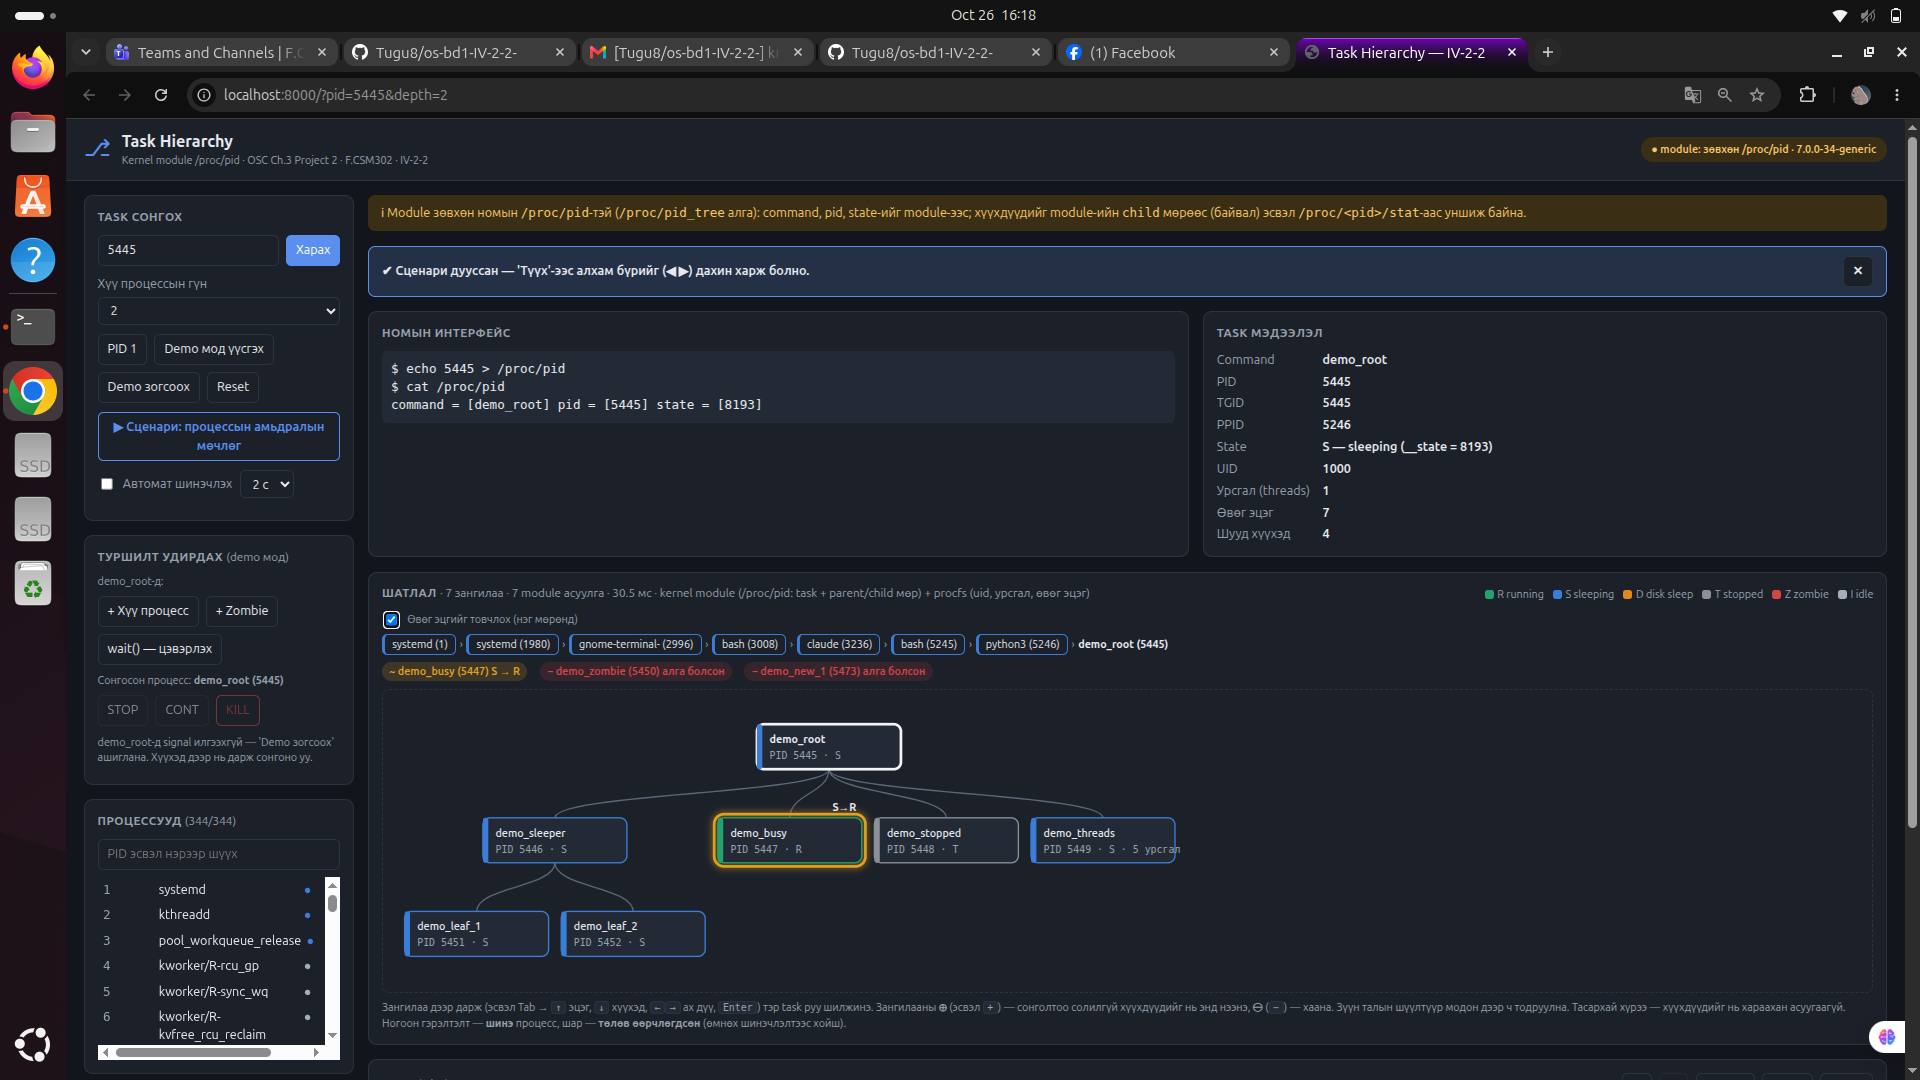
\includegraphics[width=\linewidth,height=0.4\textheight,keepaspectratio]{ui_baremetal_tree.png}
\caption{Bare-metal: \code{demo_root}-ийн мод, \code{book} горим, \code{__state = 8193}.}
\end{figure}
\begin{figure}[h!]
\centering
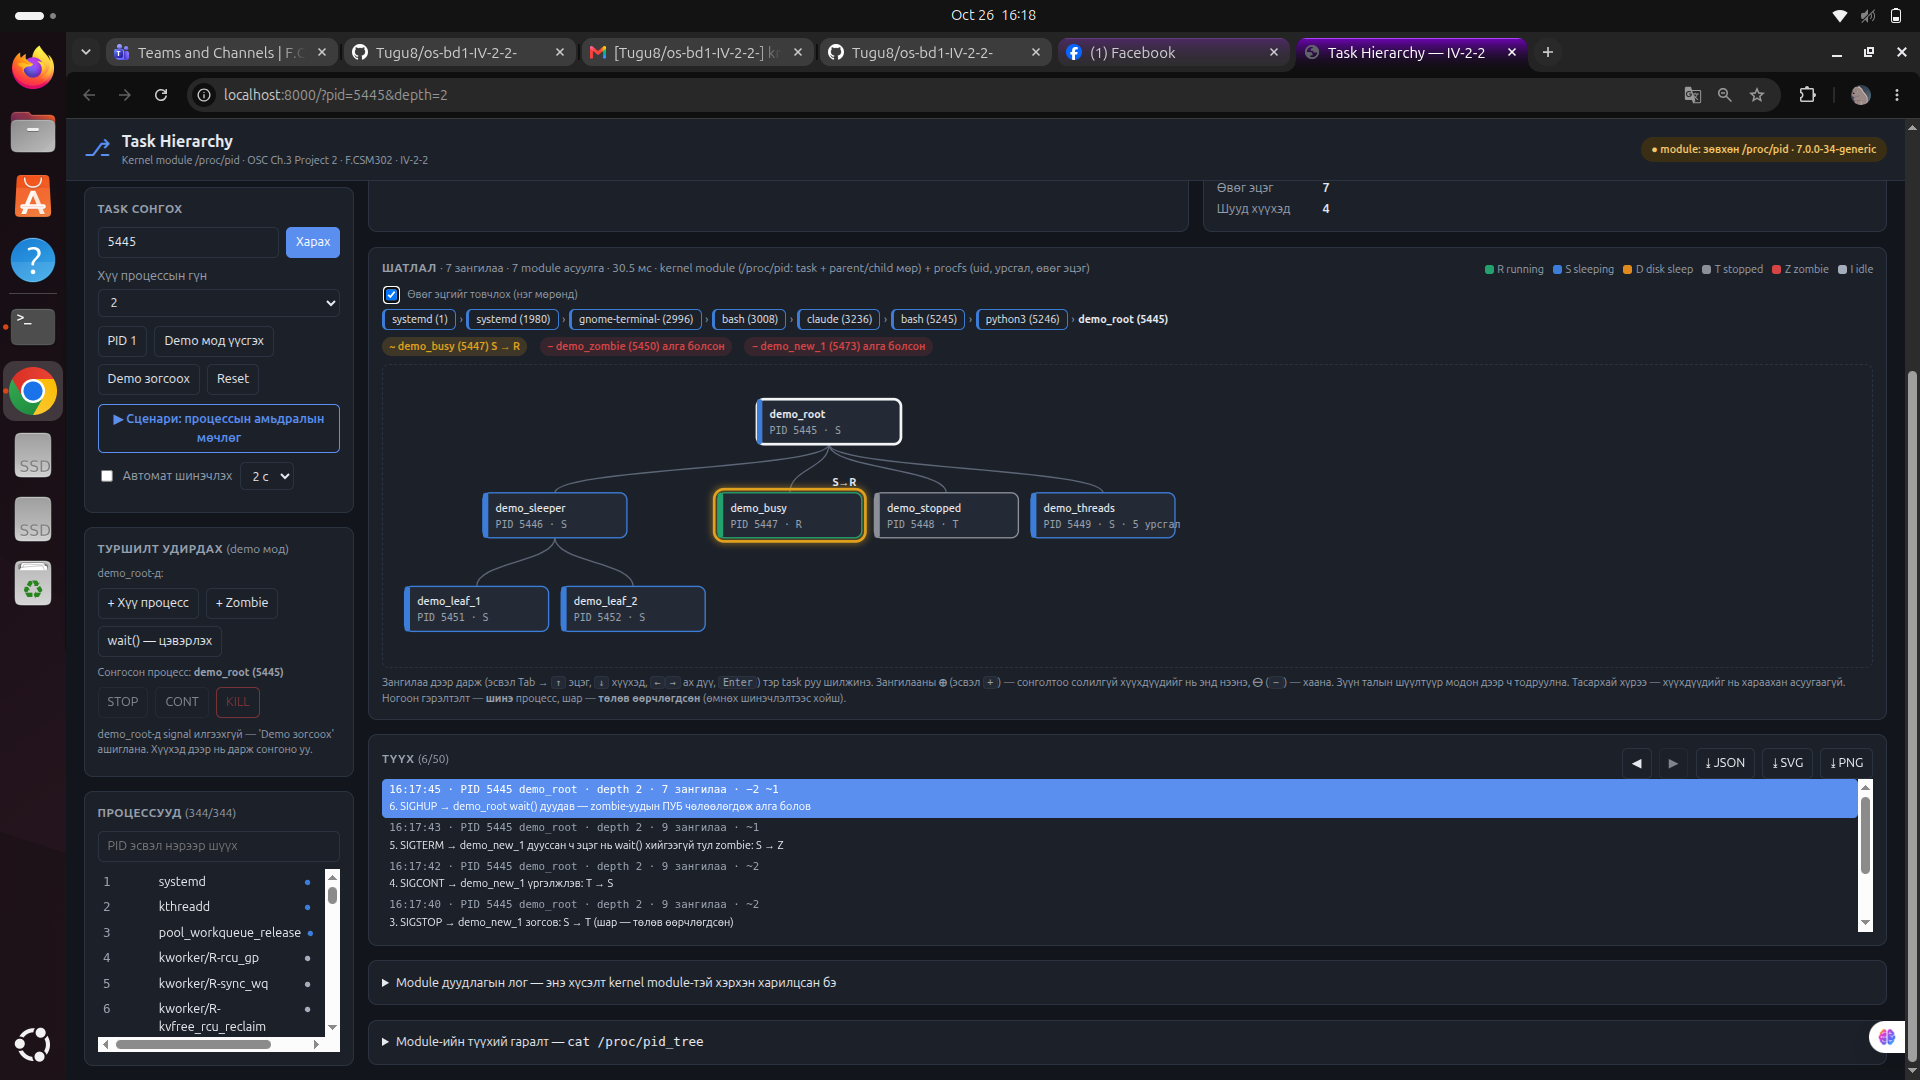
\includegraphics[width=\linewidth,height=0.4\textheight,keepaspectratio]{ui_baremetal_history.png}
\caption{Bare-metal: сценарийн түүх — SIGSTOP, SIGCONT, SIGTERM → zombie, \code{wait()}.}
\end{figure}
\begin{figure}[h!]
\centering
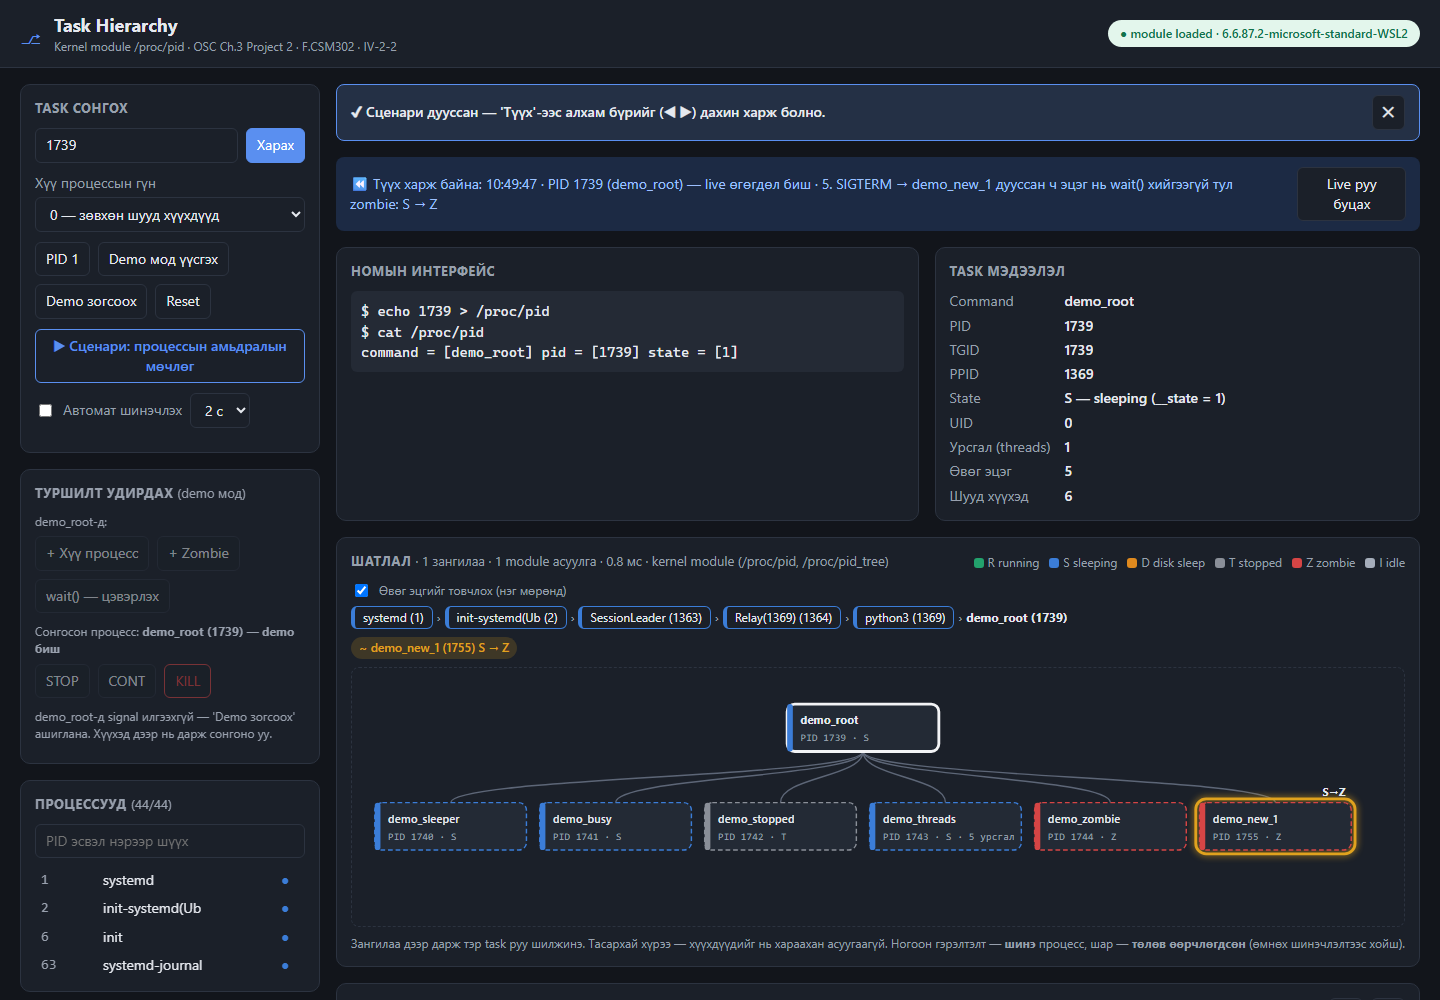
\includegraphics[width=0.49\linewidth]{step5_zombie.png}\hfill
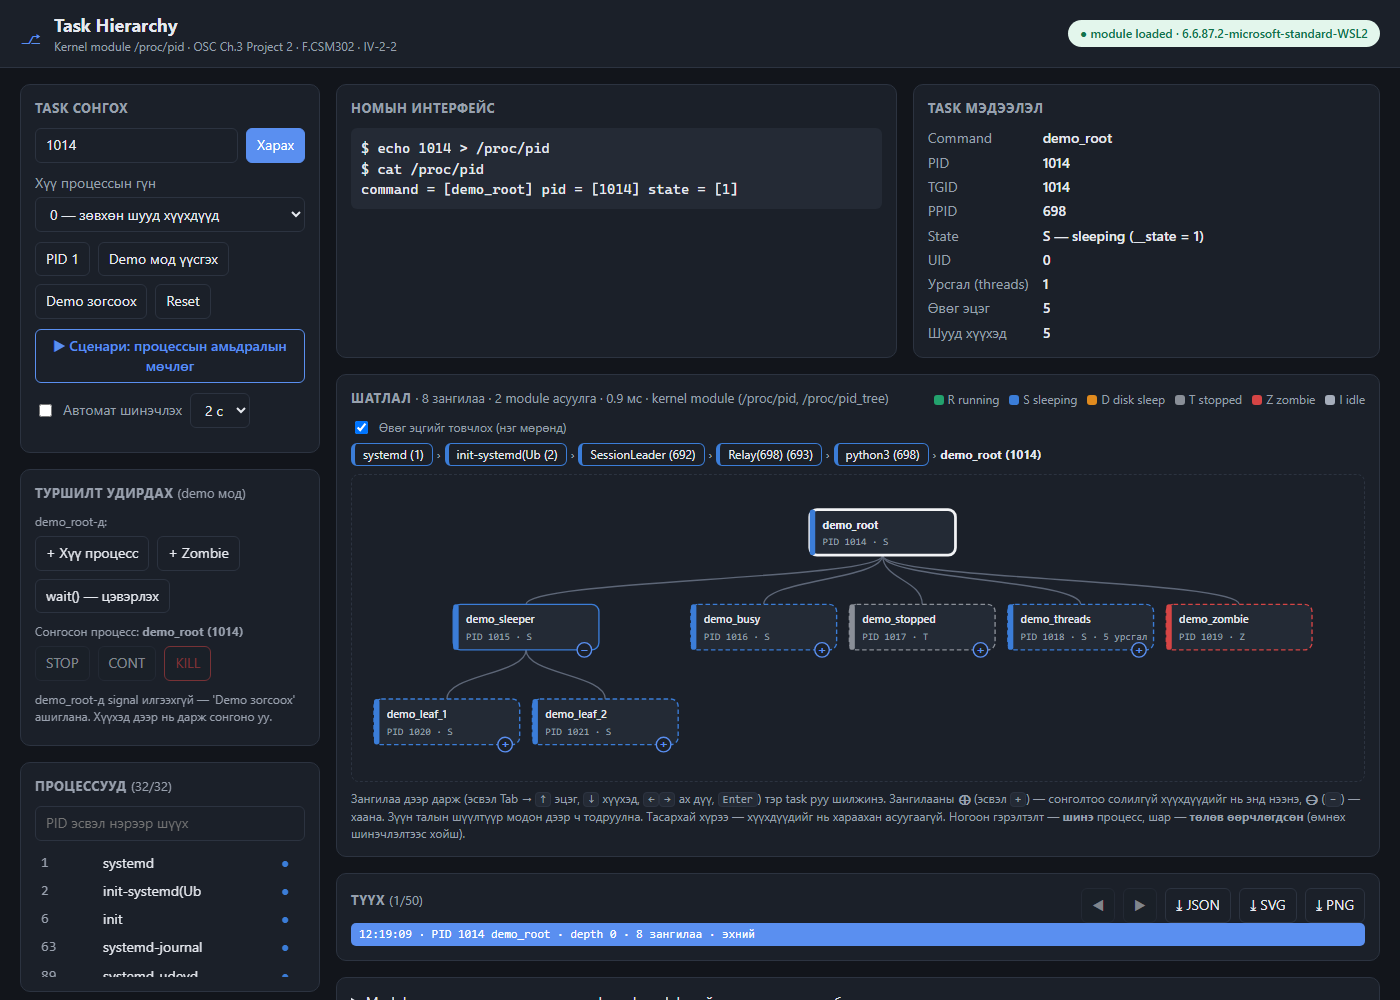
\includegraphics[width=0.49\linewidth]{expand_in_place.png}
\caption{Зүүн: SIGTERM → \code{demo_new_1} S→Z (эцэг \code{wait()} хийгээгүй). Баруун: газар дээр нь нээх (⊕/⊖), товчилсон өвөг эцэг.}
\end{figure}
\FloatBarrier

%================================================================ 9
\section{Хэлэлцүүлэг}

\textbf{Үр дүнгийн тайлбар.} Номын жишээ болон бүх захын оролт хүлээгдсэн үр дүнтэй таарсан; kernel crash, санах ойн алдагдал гараагүй. Bare-metal ба WSL2 хоёр өөр kernel (7.0 ба 6.6) дээр ижил эх код хөрвүүлэгдэж ажилласан нь \code{proc_ops}, \code{__state} API-ийн сонголт зөв болохыг харуулна.

\textbf{Туршилтаар илэрсэн, зассан алдаа.}
\begin{center}
\begin{tabular}{p{6.6cm} p{8.8cm}}
\toprule
\textbf{Асуудал} & \textbf{Засвар}\\
\midrule
WSL2-д \code{echo 1} → \code{pid = [256]}: \code{task->pid} нь global PID & \code{task_pid_vnr()} — бичигчийн namespace-ийн PID (\code{3234d12})\\
Хэсэгчлэн (8 байтаар) уншихад мөр тасрах эрсдэл (номын \code{completed} туг) & \code{seq_file} + \code{single_open}\\
UI-ийн гүн 0 ба 1 ижил мод & \code{level < depth} → \code{level <= depth}\\
Сервер зогсоход туршилтын процессууд өнчин үлдэх & \code{demo_root} эцгээ шалгаж өөрийгөө цэвэрлэнэ\\
\bottomrule
\end{tabular}
\end{center}

\textbf{Хязгаарлалт.}
\begin{itemize}[nosep]
  \item \code{l_pid} бүх хэрэглэгчид нэг; терминалаас зэрэг бичвэл бие биеийнхээ PID-ийг дарна (UI мутексээр хамгаалдаг).
  \item \code{0666} эрхтэй тул ямар ч хэрэглэгч PID бичнэ; харин \code{/proc/<pid>/stat}-д аль хэдийн нээлттэй мэдээллийг л харуулна.
  \item \code{state} нь битийн маск тул том тоо гарч болно; үсгэн төлөвийг UI procfs-оос авна.
  \item UI тогтмол хугацаанд асуудаг; хоёр шинэчлэлтийн хооронд үүсээд дууссан процесс харагдахгүй.
  \item \code{list_for_each_entry_rcu} нь \code{children} жагсаалтад хэрэглэгддэг ч албан ёсоор энэ жагсаалтыг \code{tasklist_lock} хамгаалдаг; маш их ачаалалтай үед ховор зөрүү гарч болзошгүй.
  \item Kernel < 5.14 дээр хөрвүүлэгдэхгүй; Secure Boot асаалттай бол гарын үсэг шаардана.
\end{itemize}

%================================================================ 10
\section{Дүгнэлт}

Сурах бичгийн Programming Project 2-ын бүх шаардлагыг (\code{/proc/pid} write, read, номын формат, хүчингүй PID → 0 байт) хэрэгжүүлж, task hierarchy дүрслэлд зориулан эцэг, хүүхдийн мөрөөр өргөтгөсөн. 2-р бүлгийн бэлтгэл module-ууд орчныг шалгана. Интерактив UI нь бодит module-тай \code{/proc/pid}-ээр холбогдож, процессын амьдралын мөчлөгийг (fork, stop, zombie, wait) бодит цагт харуулна. Bare-metal ба WSL2 дээрх 60 гаруй автомат шалгалт, 10 гар тестээр зөв ажиллагааг нотолж, PID namespace-ийн алдааг илрүүлж зассан. Өөр компьютер дээр дахин ажиллуулах алхмыг \code{docs/Manual.md} (\code{IV-2-2_Manual.pdf}) болон README-ийн Quick Start-д бичсэн.

%================================================================ Материал
\section*{Ашигласан материал}
\addcontentsline{toc}{section}{Ашигласан материал}
\begin{enumerate}[nosep, label={[\arabic*]}]
  \item A. Silberschatz, P. B. Galvin, G. Gagne. \emph{Operating System Concepts}, 10th ed. Wiley, 2018. — Ch.2–3 Programming Projects, §3.1–3.3, §6.7.
  \item Linux kernel source — \code{include/linux/sched.h}, \code{include/linux/proc_fs.h}, \code{fs/seq_file.c}, \code{kernel/pid.c}. \url{https://elixir.bootlin.com/linux/latest/source}
  \item The Linux Kernel documentation — ``The /proc Filesystem'', ``seq\_file interface'', ``RCU concepts''. \url{https://docs.kernel.org/}
  \item P. J. Salzman et al. \emph{The Linux Kernel Module Programming Guide}. \url{https://sysprog21.github.io/lkmpg/}
  \item F.CSM302 лекц (Г. Ганбат): Lec3 Процесс, Lec4 Урсгал, Lec6 Синхрончлол; OS\_BD1\_Guide.
  \item Python 3 documentation — \code{http.server}, \code{threading}. \url{https://docs.python.org/3/}
\end{enumerate}

\textbf{Бэлэн код, AI ашиглалт.} Kernel module нь номын Programming Project-ийн skeleton (\code{proc_ops}, \code{kmalloc}, \code{copy_from_user}, \code{kstrtol}, \code{pid_task}, \code{find_vpid}) дээр суурилсан. UI (\code{src/ui/}), бэлтгэл module-ууд (\code{src/prereq/}), README/CONTRIBUTING, Manual §A болон энэ тайланг B190910014 Claude (Anthropic) AI туслахын тусламжтайгаар бэлтгэсэн; хариуцсан гишүүд кодыг уншиж, ажиллуулж, бодит орчинд туршиж шалгана. Гадны программын сан ашиглаагүй.

%================================================================ Хавсралт
\appendix
\section*{Хавсралт A. Ажлын төлөвлөгөө}
\addcontentsline{toc}{section}{Хавсралт A. Ажлын төлөвлөгөө}
\begin{center}
\begin{tabular}{l p{11.5cm}}
\toprule
Хуваарилалтын код & IV-2-2\\
Төсөл & Linux Kernel Module for Task Information\\
Repository & \url{https://github.com/Tugu8/os-bd1-IV-2-2-}\\
Хэл/сан/орчин & C (Linux kernel module), Python 3 стандарт сан + HTML/CSS/JS; Ubuntu bare-metal\\
Үндсэн дүрслэл & Task hierarchy (parent – task – children мод)\\
Шүүмжлэх баг & IV-2-5 (Sudoku Solution Validator)\\
\bottomrule
\end{tabular}

\medskip
\begin{tabular}{l p{8.8cm} p{3.6cm}}
\toprule
\textbf{Гишүүн} & \textbf{Хариуцах ажил} & \textbf{Commit/file}\\
\midrule
B242270047 & Үндсэн kernel module: write, read, parent/children өргөтгөл, \code{proc_ops}, \code{__state}; Release & \code{src/kmod/}\\
B190910014 & Interactive UI: PID оруулах/сонгох, мод, төлөвийн өнгө, refresh/reset, алдааны мэдэгдэл & \code{src/ui/}\\
B210930842 & 2-р бүлгийн бэлтгэл module, build орчин, Operational manual & \code{src/prereq/}, \code{docs/Manual.md} §A\\
B231910003 & Туршилт: номын жишээ, boundary/error тест & \code{tests/}\\
B232270108 & Үндсэн тайлан (Report.pdf) & \code{report/}\\
B241940099 & Хэрэглэгчийн manual, README Quick Start, БД1 пост, IV-2-5-ийн шүүмж & \code{docs/Manual.md} §B, \code{review/}\\
\bottomrule
\end{tabular}

\medskip
\begin{tabular}{c p{6cm} p{7.4cm}}
\toprule
\textbf{Тест} & \textbf{Оролт/нөхцөл} & \textbf{Хүлээгдсэн үр дүн}\\
\midrule
1 & Ажиллаж буй bash-ийн PID & \code{command = [bash] pid = [...] state = [...]}\\
2 & PID 1 (systemd/init) & Мэдээлэл гарч, children олон байна\\
3 & Байхгүй PID (жишээ 999999) & Read 0 буцаана, UI ойлгомжтой алдаа харуулна\\
4 & Тоо биш оролт (\code{abc}), сөрөг тоо & Write алдаа буцаана, kernel crash гарахгүй\\
5 & Child process үүсгээд түүний parent-ийн PID & Мод дээр шинэ child харагдана\\
\bottomrule
\end{tabular}
\end{center}

\end{document}
